\subsubsection{Overview}
Data control board (DCB) are intented to be a part of the LHCb upstream tracker
upgrade.
There is one master GBTx ASIC, and 6 data GBTx ASICs per board.
DCB is much less flexible than GBTx DB, because it serves only one purpose:
Receive SALT elink data then transmit that data to the counting room.

So far, we have been able to repeat PRBS test on DCBs:
Programming the master, then programming data GBTxs, then instruct them to
generate PRBS data, and verify generated data by MiniDAQ.

\autoref{fig:dcb_layout} shows the layout of an actual DCB board.
%GBTx ASICs layout are marked on the figure directly.
Optical fiber grouping are marked by the \texttt{OMDBXX} label. For example,
\texttt{OMDB23} means that data GBTxs 2 and 3 are connected to this mezzanine.

A DCB requires 4 optical mezzanines (not shown here) to function properly.
As said above, DCB is less flexible, and there will be only \emph{one}
configuration for DCBs.
All DCBs shipped with UMD LHCb group will have its hardware jumpers
pre-configured.

\begin{figure}[!ht]
\centering
\begin{tikzpicture}
    \node [anchor=south west] (main) {
            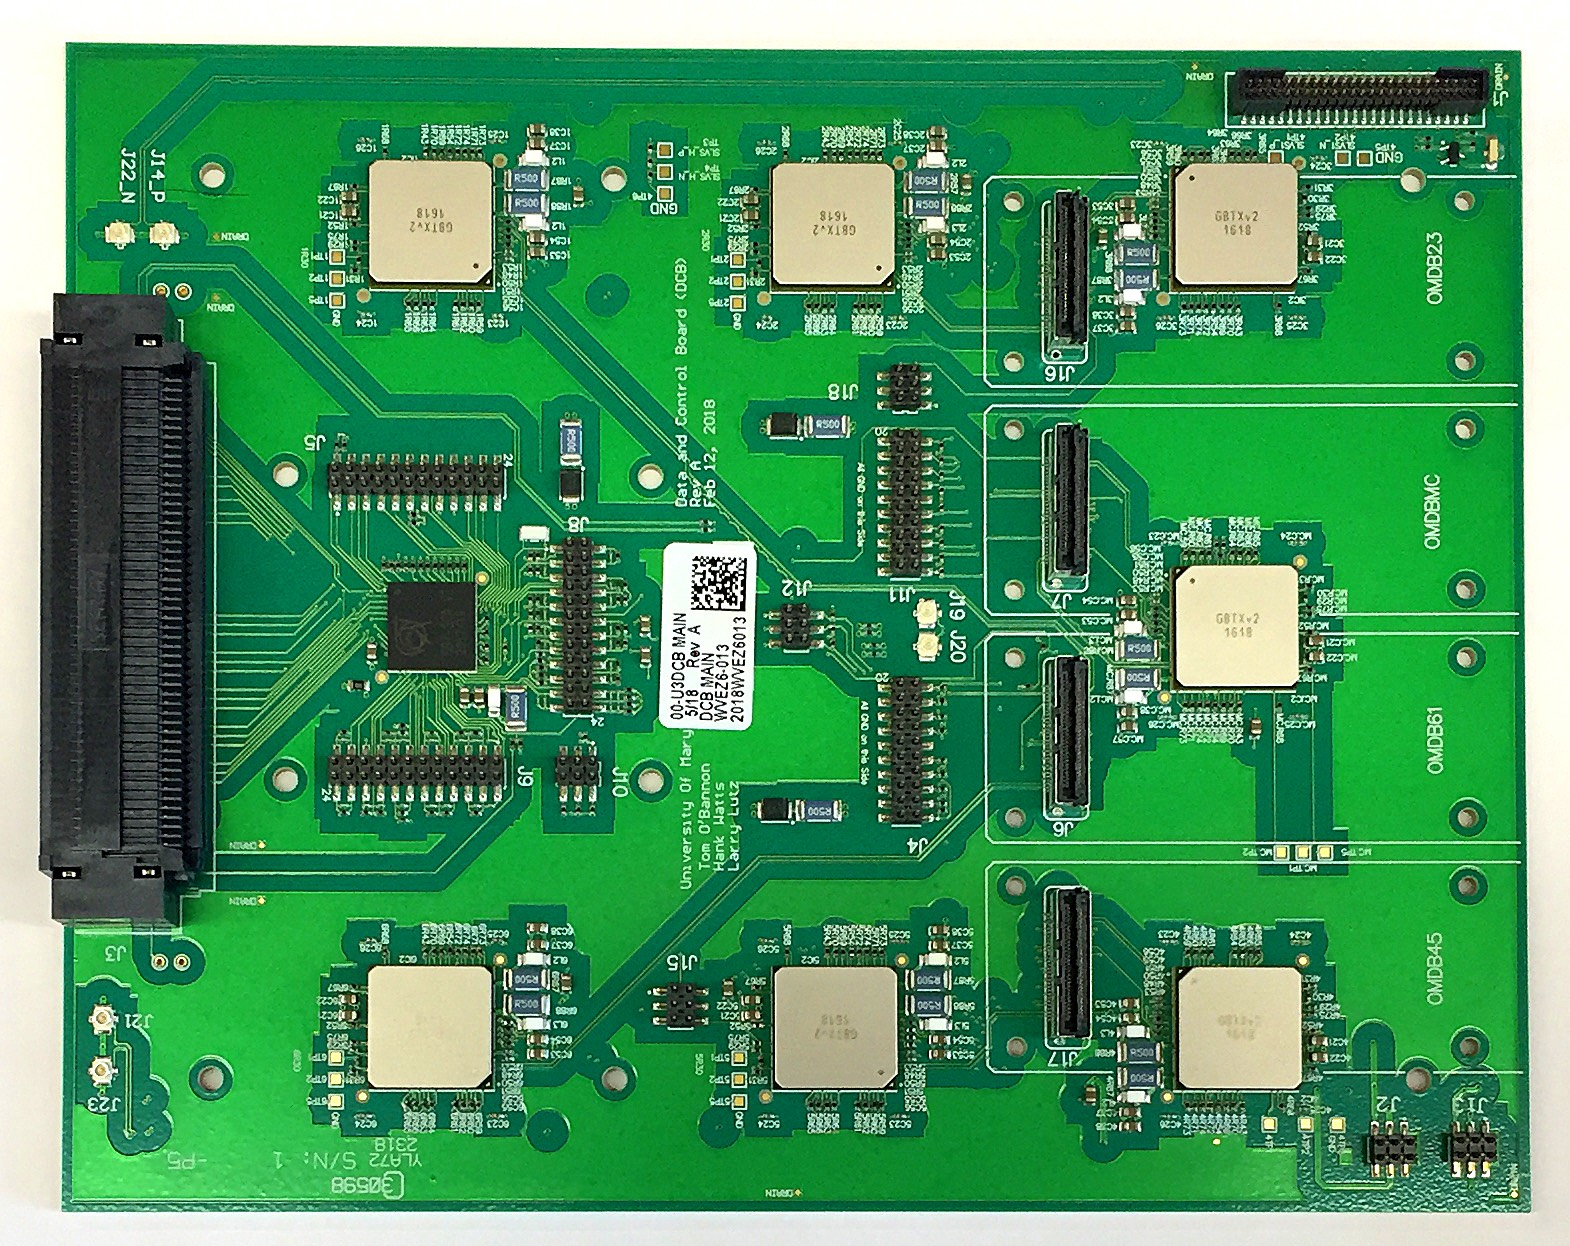
\includegraphics[width=0.9\linewidth]{res/dcb_layout.png}
        };
    \begin{scope}[x=(main.south east),y=(main.north west)]
        \draw [fill=none,red,very thick] (0.24,0.76) rectangle ++(0.0813,0.1)
            node [pos=.5] {\tiny\texttt{data 1}};
        \draw [fill=none,red,very thick] (0.24,0.135) rectangle ++(0.0813,0.1)
            node [pos=.5] {\tiny\texttt{data 6}};

        \draw [fill=none,blue,very thick] (0.49,0.76) rectangle ++(0.0813,0.1)
            node [pos=.5] {\tiny\texttt{data 2}};
        \draw [fill=none,blue,very thick] (0.74,0.76) rectangle ++(0.0813,0.1)
            node [pos=.5] {\tiny\texttt{data 3}};

        \draw [fill=none,magenta,very thick] (0.74,0.135)
                rectangle ++(0.0813,0.1)
            node [pos=.5] {\tiny\texttt{data 4}};
        \draw [fill=none,magenta,very thick] (0.49,0.135)
                rectangle ++(0.0813,0.1)
            node [pos=.5] {\tiny\texttt{data 5}};

        \draw [fill=none,orange,very thick] (0.74,0.448) rectangle ++(0.0813,0.1)
            node [pos=.5] {\tiny\texttt{master}};
    \end{scope}
\end{tikzpicture}
\caption{Pilot-run DCB layout.}
\label{fig:dcb_layout}
\end{figure}
